\chapter{Acciai Speciali da Costruzione}\label{chp:SpecCostruzione}
Sono acciai che vengono caratterizzati tramite la composizione chimica
infatti questi acciai sono spesso trattati con successivi
trattamenti termici prima di essere messi in opera.

In generale vengono classificati tra:
\begin{itemize}
\item Acciai da costruzione propriamente detti;
\item Acciai inossidabili;
\item Acciai da utensili.
\end{itemize}

\section{Acciai speciali da costruzione propriamente detti}
Sono acciai calmati che spesso vengono legati con diversi elementi che donano
particolari capacità tipo: temprabilità, tenacità, buon compromesso tra
tenacità e resistenza meccanica, resistenza all'usura e altre\dots
Come accennato prima spesso vengono applicati dopo aver subito un trattamento 
termico (tempra + rinvenimento).
In genere son impiegati per applicazioni che devono resistere a elevate 
sollecitazioni dinamiche e statiche.

Questi vengono ulteriormente suddivisi secondo l'impiego.
\begin{itemize}
\item Acciai da bonifica,
\item Acciai da cementazione,
\item Acciai da nitrurazione,
\item Acciai per molle,
\item Acciai per cuscinetti,
\item Acciai "automatici",
\item Altri (acciai da bulloneria)\dots
\end{itemize}

In generale sulle schede tecniche degli acciai si trovano degli intervalli 
con dei valori nominali di composizione chimica. Alcuni riferimenti si posso 
trovare nelle varie normative tipo la \texttt{UNI EN 10027} ed eventuali 
normative prodotto aggiuntive.
Inoltre, viene accompagnato con la lista dei trattamenti termici che il 
materiale ha subito ed eventuali caratteristiche meccaniche che si sono 
raggiunte.

Le motivazioni dietro a questa non precisa specificità della composizione
del materiale è dovuta al fatto che ci sono diverse variabili che incorrono 
per il raggiungimento degli obbiettivi meccanici.
Dunque è difficile effettivamente stimare la composizione chimica.

\subsection{Acciai da Bonifica}
Gli acciai da bonifica sono acciai che subiscono un trattamento termico
tipo quello in figura \ref{fig:AccBonifica}.

\begin{figure}
\centering
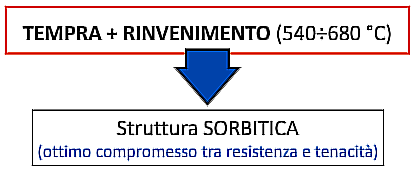
\includegraphics[width = 0.5\textwidth]{AccBonifica}
\caption{Trattamento termico per gli acciai da bonifica}
\label{fig:AccBonifica}
\end{figure}

Gli acciai da bonifica sono adatti, in relazione alla loro composizione 
chimica, per sopportare sforzi, urti e vibrazioni, infatti di solito
si realizzano:
\begin{itemize}
\item Alberi motore,
\item assi,
\item pignoni,
\item bielle,
\item rotismi,
\item ecc\dots
\end{itemize}
Infatti sono parti della macchina che devono possedere delle buone
resistenze a carichi elevati ed alta tenacità.